\subsubsection{Artificial Neural Networks}
	An Artificial Neural Network (ANN) \cite{mcculloch1943logical} is a mathematical computational model, whose development was inspired by cognitional processes in a biological brain. AN Networks typically consist of numerous interconnected input and output information units. The form of connectivity between these units embodies the connection strength, in a fashion similar to how neurons are linked in the brain. ANNs are predominantly used in Cognitive Sciences and related applications, of which Artificial Intelligence is a prominent example. Common tasks for such systems are character and facial recognition, financial markets prediction and text mining among other uses.
	
	\paragraph{Intuition}
		A neural network is composed of linked processors called Perceprtons (combination of preception and neurons). Each Perceprton is capable of executing simplistic mathematical operations, however when combined into networks, they are capable of elaborate and sophisticated problem solving. Any given Perceptron receives inputs $ i $ with according weights $ w $. These weighted inputs (products) are then summed up. When said sum exceeds a threshold value $ T $, the output $ O $ is equal to one and zero otherwise, as in [\ref{ann_neuron_sumprod}]. This operation mimics the operation of a biological neuron, which releases an electric signal when its agitation transcends a certain limit.
	
	\begin{equation}
		\langle i,w \rangle = \sum_j i_j w_j = 
			\begin{cases}
				1 \ \ \text{,  } \sum_j i_j w_j \geq T \\
				0 \ \ \text{,  } \sum_j i_j w_j < T 
			\end{cases}
		 = O
		\label{ann_neuron_sumprod}
	\end{equation}
	
	\begin{figure}[h]
		\centering
		\captionsetup{width=0.8\textwidth}
		\begin{tikzpicture}[
init/.style={
  draw,
  circle,
  inner sep=2pt,
  font=\Huge,
  join = by -latex
},
squa/.style={
  draw,
  inner sep=2pt,
  font=\Large,
  join = by -latex
},
start chain=2,node distance=13mm
]
\node[on chain=2] 
  (x2) {$x_2$};
\node[on chain=2,join=by o-latex] 
  {$w_2$};
\node[on chain=2,init] (sigma) 
  {$\displaystyle\Sigma$};
\node[on chain=2,squa,label=above:{\parbox{2cm}{\centering Activation \\ function}}]   
  {$f$};
\node[on chain=2,label=above:Output,join=by -latex] 
  {$y$};
\begin{scope}[start chain=1]
\node[on chain=1] at (0,1.5cm) 
  (x1) {$x_1$};
\node[on chain=1,join=by o-latex] 
  (w1) {$w_1$};
\end{scope}
\begin{scope}[start chain=3]
\node[on chain=3] at (0,-1.5cm) 
  (x3) {$x_3$};
\node[on chain=3,label=below:Weights,join=by o-latex] 
  (w3) {$w_3$};
\end{scope}
\node[label=above:\parbox{2cm}{\centering Bias \\ $b$}] at (sigma|-w1) (b) {};

\draw[-latex] (w1) -- (sigma);
\draw[-latex] (w3) -- (sigma);
\draw[o-latex] (b) -- (sigma);

\draw[decorate,decoration={brace,mirror}] (x1.north west) -- node[left=10pt] {Inputs} (x3.south west);
\end{tikzpicture}
		%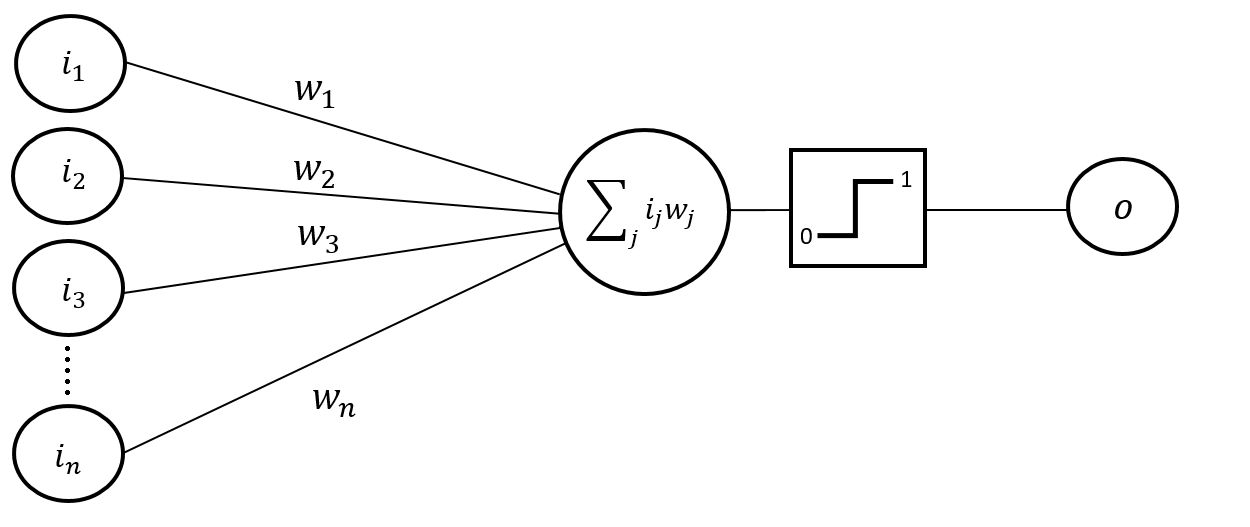
\includegraphics[width=0.8\textwidth]{ANN_percept.png}
		\caption[ANN Perceptron]{
			\footnotesize{
				Structure of a Perceptron with 3 input nodes $ x_i $ and output $ y $. Output 1 when threshold is surpassed and zero otherwise.
			}
		} 
		\label{ANN_percept}
	\end{figure}
	
	The organization of Perceptrons is crucial to the networks operation. The input weights are the ones, which determine the pattern to be recognized \cite{bishop1995neural}. Therefore, the prime objective when constructing an ANN is determining proper values for the weights. The Perceptrons are used as logical gateway, which can carry out the "AND" and "OR" operations. A major obstacle in the early days of ANNs was the inability to construct  a "XOR" (exclusive OR) logical gate, irregardless of the weights on the inputs. This difficulty was later overcome with the introduction of multi-layered ANN.
	
	Multi-layered ANNs consist of several layers of Perceptrons. All layers except the first (input layer) and the last (output layer) receive their inputs from the lower level of Perceptrons and output into the higher layer, which in turn uses this output as its input. It was demonstrated that a "XOR" gateway could be constructed using a 3-layered network [\ref{ANN_XOR}].
	
	\begin{figure}[h]
		\resizebox{0.9 \textwidth}{!}{
		\begin{minipage}[b]{0.4\linewidth}
			\begin{tabular}{cc|c}
				 \\ \\ \\
				\hline\hline
				Input$_1 $ & Input$_2 $ & Output \\
				\hline
				0 & 0 & 0\\
				1 & 0 & 1\\
				0 & 1 & 1\\
				1 & 1 & 0\\
				\hline\hline
			\end{tabular}
		\end{minipage}	
		\begin{minipage}[c]{0.56\linewidth}
			\centering
			\input{images/perceptron.eps_tex}
		\end{minipage}
		}
		\captionsetup{width=0.8\textwidth}
		\caption[ANN XOR Perceptron-Network]{
			\footnotesize{
				A three layer Network, creating a XOR gateway.
			}
		} 
		\label{ANN_XOR}
	\end{figure}	
	
	%\begin{tikzpicture}[
plain/.style={
  draw=none,
  fill=none,
  },
net/.style={
  matrix of nodes,
  nodes={
    draw,
    circle,
    inner sep=10pt
    },
  nodes in empty cells,
  column sep=2cm,
  row sep=-9pt
  },
>=latex
]
\matrix[net] (mat)
{
|[plain]| \parbox{1.3cm}{\centering Input\\layer} & |[plain]| \parbox{1.3cm}{\centering Hidden\\layer} & |[plain]| \parbox{1.3cm}{\centering Output\\layer} \\
& |[plain]| \\ |[plain]| & \\
& |[plain]| \\ |[plain]| & |[plain]| \\
& 	    			   	 & \\ |[plain]|   & |[plain]| \\
& |[plain]| \\ |[plain]| & \\
& |[plain]| \\    
};
\foreach \ai [count=\mi ]in {2,4,...,10}
  \draw[<-] (mat-\ai-1) -- node[above] {Input \mi} +(-2cm,0);
\foreach \ai in {2,4,...,10}
{\foreach \aii in {3,6,9}
  \draw[->] (mat-\ai-1) -- (mat-\aii-2);
}
\foreach \ai in {3,6,9}
  \draw[->] (mat-\ai-2) -- (mat-6-3);
\draw[->] (mat-6-3) -- node[above] {Ouput} +(2cm,0);
\end{tikzpicture}


	
	\paragraph{Classification}
		The type of network used most commonly for classification is a Multilayer Perceptron Network (MLP). This falls into the category of feedforward ANNs. A feedforward network is one, which prohibits cycles between its nodes. Thus each layer only outputs information to the next layer, and not to the ones which came before. Typically, a non-linear sigmoid function is used for activation rather than a binary step function as described in [\ref{ANN_percept}]. A sigmoid function [\ref{ann_sigmoid}] (often called a Soft-Step) or another continuous function are usually used, since ultimately the algorithm will have to calculate gradients to maximize or minimize an optimization function. Therefore this function should be continuous, differentiable and Real-valued.
		
		\begin{equation}
			\phi(x) = \frac{1}{1+ e^{-x}}
			\label{ann_sigmoid}
		\end{equation}
			
		\par
		
		The network is than optimized through the process of \textbf{Backpropogation} of errors. During the backwards propagation the initial weights of all the axons (input nodes of a neuron) weights are determined at random. Subsequently, the optimization problem is set by measuring the aggregate error terms in classification (misclassification). This error is calculated as a function of all afore mentioned weights. Next, the aggregate error function must to be minimized by observing the contribution of each weight to the error and reducing it. Finally, the gradient (derivative in vector space) is derived and the weights are adjusted by $ \Delta w $ respectively as shown in  figure \ref{ANN_backprop}. This process is repeated, pending we no longer get improvement (lower error terms) or the error reduction is lower than a predetermined threshold.
		
		\begin{figure}[h]
			\centering
			\captionsetup{width=0.8\textwidth}
			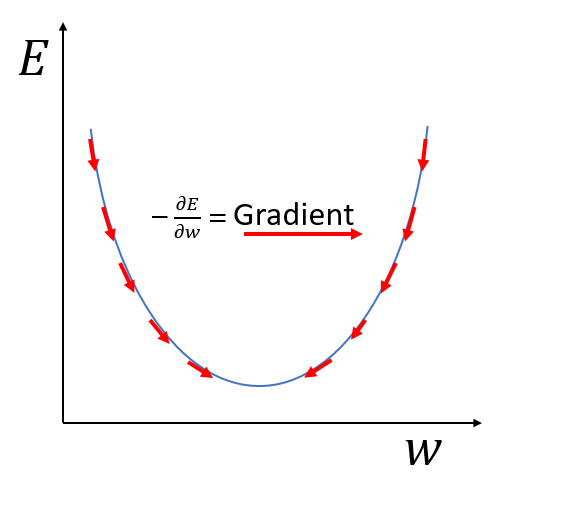
\includegraphics[width=0.5\textwidth]{grad_desc.png}
			\caption[ANN Gradient Descent]{
				\footnotesize{
					A descent down the error function, taking gradients of $ w $ to calculate the steps.
				}
			} 
			\label{ANN_backprop}
		\end{figure}
	
	\paragraph{Stochastic Gradient Descent}
		In the basic variant of ANN's, an objective function is optimized by tuning the weights in a manner which reduces the error term gradually with each iteration. In every repetition the weights are adjusted by $ \Delta w $ according to the gradient for each weight over all the observations. Every repetition  requires the calculation of the function's derivatives with respect to every data point and their summation within every iteration. This base method is also referred to as Batch Gradient Descent (BGD). This means, that in order to tune a weight $ w_j $ we must go through all its derivatives in the gradient and sum them up.  Applying this technique requires us to derive the function $ m \cdot n $ times in each step of the algorithm, with $ m $ and $ n $ being the number of data points and the set size of features respectively. The problem with this procedure is its computational costliness which increases as the data set grows larger. Therefore, the standard BGD approach scales poorly. We can hence modify the algorithm using a method called Stochastic Gradient Descent (SGD) to address scalability issues.
		
		\par
	
		To carry out SGD we first shuffle the training dataset to avoid any inherit order or structure present in the dataset. Subsequently, we derive each of the weight modification and adjust after each derivation before continuing to the next data point. Finally, we repeat this process for each data point. Noteworthy is that we are now adjusting after each derivation instead for all derivations of a data point. Therefore, the descent tempo is now $ (m \cdot n) \ \frac{\text{improvements}}{\text{algorithm round}}$ as compared to the tempo $(n) \ \frac{\text{improvements}}{\text{algorithm round}}$ of BGD. Hence, SGD progresses $ m $ times as fast as BGD. Additionally, the loop over all the data points can be repeated more than once for better results.
		
		\par
		
		Since each adjustment is being made for a single data point at a time, it is much more likely that the adjustment is not actually an improvement and possibly takes us further away (or not nearer) from the global minimum. Nonetheless, the algorithm does converge to the extremum and faster at that, then the BGD approach.  Figure [\ref{ann_sto_grad_desc}] illustrates graphically the convergence of both SGD and BGD. The stochastic approach is clearly recognizable with its "squiggly" line. One notable problem with this algorithm is that it might continuously overshoot the local minimum due to its high variance.
		
		\begin{figure}[H]
			\centering
			\captionsetup{width=0.8\textwidth}
			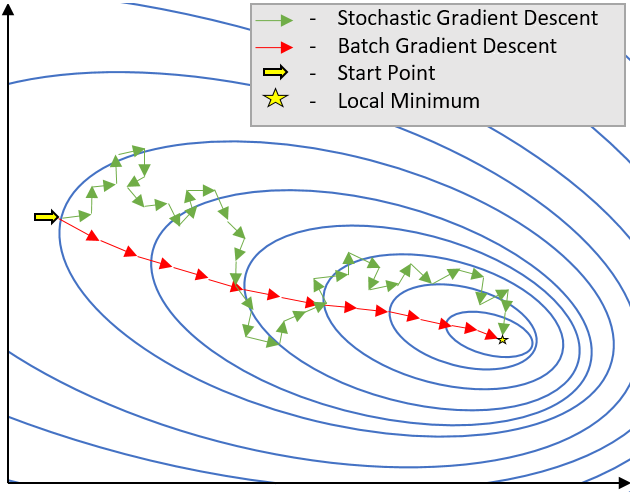
\includegraphics[width=0.4\textwidth]{sto_grad_desc.png}
			\caption[Batch and Stochastic Gradient Descent]{
				\footnotesize{
					A comparison of the Batch and Stochastic Gradient Descent Approaches 
				}
			} 
			\label{ann_sto_grad_desc}
		\end{figure}
	
		In the example above, an SGD approach is described, in which we fit the weights for a single observation at a time. Another possible modification is to take minute batches of observations and fitting the algorithm on them instead of the entire dataset. This approach is also known as Mini-Batch Gradient Descent and combines the best of both approaches, since it simultaneously addresses the overshooting complication of SGD and is speedier than BGD. Thus, by adjusting the batch size one can control the trade-off between speed and accuracy, where a larger batch results in a more accurate step, but the computation time will also increase. 
		
		\par
		
		The mechanism of Stochastic Gradient Descent, at its core, is extremely inaccurate on a single step basis. This is due to the probability of improvement being much lower when compared to Batch Gradient Descent. However, this is compensated for with a more rapid improvement rate, making the accumulated advancement catch up and overtake that of the normal scenario. The heightened convergence pace is what makes this approach more suitable for classification with extensive training data sets.
		
	\paragraph{Adaptive Moment Estimation}
		ADAM is another approach often used in tandem with SGD. Using ADAM we calculate the first (mean) and second (variance) moment of the gradients and modify the step size for each parameter (feature) in accordance with its frequency. Therefore, the update size is usually more significant for infrequent parameters and more fine for frequently occurring ones.
			
		 

				
				